\documentclass[11pt]{article}

%FOR SCRIBES: Please change the next three lines to reflect the correct
%FOR SCRIBES: lecture number, name, and date.
\newcommand{\lecturenumber}{4}
\newcommand{\scribename}{Abdullah AlJasser, Andrew McBurnett, Robert Terpin}
\newcommand{\lecturedate}{5/25/23} 

\usepackage{subfigure}
\usepackage{color}
\usepackage{url}
\usepackage{graphicx}
\usepackage{fullpage}
\newcommand{\etal}{{\em et al.}}
\newcommand{\qed}{\mbox{}\hspace*{\fill}\nolinebreak\mbox{$\rule{0.6em}{0.6em}$}}
\newcommand{\expect}{{\bf \mbox{\bf E}}}
\newcommand{\prob}{{\bf \mbox{\bf Pr}}}

%--------------------------- Commands and Environments I added -----------------
\usepackage[english]{babel}
\usepackage{amssymb}
\usepackage{amsmath}
\usepackage{fancyhdr}
\renewcommand{\baselinestretch}{1.10}
%%      Fonts:
%%---------------------------------------------------------------------------
\newfont{\bssten}{cmssbx10}
\newfont{\bssnine}{cmssbx10 scaled 900}
\newfont{\bssdoz}{cmssbx10 scaled 1200}

%---------------------------------------------------------------------------
\newcounter{topic} \setcounter{topic}{0}
\newcommand{\topic}[1]{\par \refstepcounter{topic} {\bssdoz \arabic{topic}.~ #1} \par}
%\newcommand{\topic}[1]{\par \refstepcounter{topic} \vs{2ex} {\bssdoz \arabic{topic}.~ #1} \par \vs{1ex}}

%------------------------------ end of new commands and evironments ------------

\definecolor{gray}{rgb}{0.5,0.5,0.5}
\newcommand{\comment}[1]{{\color{gray}[\textsf{#1}]}}
\newcommand{\redospace}{\small\renewcommand{\baselinestretch}{1.5}\normalsize}
\newcommand{\undospace}{\small\renewcommand{\baselinestretch}{1}\normalsize}
\newtheorem{theorem}{Theorem}[section]
\newtheorem{lemma}[theorem]{Lemma}
%----------------------------- some other things I added ---------------------
\newtheorem{claim}[theorem]{Claim}
\newtheorem{example}[theorem]{Example}
\newtheorem{protocol}[theorem]{Protocol}
%----------------------------------------------------------------------------
\newtheorem{corollary}[theorem]{Corollary}
\newtheorem{definition}{Definition}[section]
\newtheorem{remark}[definition]{Remark}
\newtheorem{conjecture}[theorem]{Conjecture}
\newtheorem{proposition}[theorem]{Proposition}
\newenvironment{proof}{{\bf Proof:}}{$\qed$\par}
\newenvironment{proofof}[1]{{\bf Proof of #1:}}{$\qed$\par}
\newenvironment{proofsketch}{{\sc{Proof Outline:}}}{$\qed$\par}

\usepackage{hyperref}
\hypersetup{
bookmarksnumbered
}

\usepackage{tikz}
\usetikzlibrary{positioning}

\begin{document}
\begin{center}
\framebox{\parbox{6.5in}{
{\bf{CS 3510: Design and Analysis of Algorithms, Summer 2023}}\\
Instructor:
He Jia, Georgia Institute of Technology.\\\ \\
{\bf Lecture \lecturenumber, \lecturedate. Scribed by \scribename.}
}}
\ \\
\end{center}
\setcounter{section}{\lecturenumber}
%FOR SCRIBES: ---------- Begin Scribing Here ------------------------
\setcounter{section}{0}

\section{Poll Questions}

\subsection{Questions}
\begin{itemize}
    \item How many distinct points are needed to uniquely determine a degree-k polynomial?
    \begin{itemize}
        \item 2
        \item k-1
        \item k
        \item k+1
    \end{itemize}
    \item How many coefficients are needed to uniquely determine a degree-k polynomial?
    \begin{itemize}
        \item 2
        \item k-1
        \item k
        \item k+1
    \end{itemize}
    \item What is the degree of the product of two polynomials of degree k?
    \begin{itemize}
        \item k
        \item k+1
        \item 2k
        \item $k^2$
    \end{itemize}
    \item How many complex roots does $z^n=1$ have?
    \begin{itemize}
        \item 1
        \item 1 or 2
        \item n
        \item n+1
    \end{itemize}
\end{itemize}

\subsection{Answers}
\begin{itemize}
    \item How many distinct points are needed to uniquely determine a degree-k polynomial?
    \begin{itemize}
        \item k+1
    \end{itemize}
    \item How many coefficients are needed to uniquely determine a degree-k polynomial?
    \begin{itemize}
        \item k+1
    \end{itemize}
    \item What is the degree of the product of two polynomials of degree k?
    \begin{itemize}
        \item 2k
    \end{itemize}
    \item How many complex roots does $z^n=1$ have?
    \begin{itemize}
        \item n
    \end{itemize}
\end{itemize}

\section{Recap}

\subsection{Polynomial Multiplication Process}
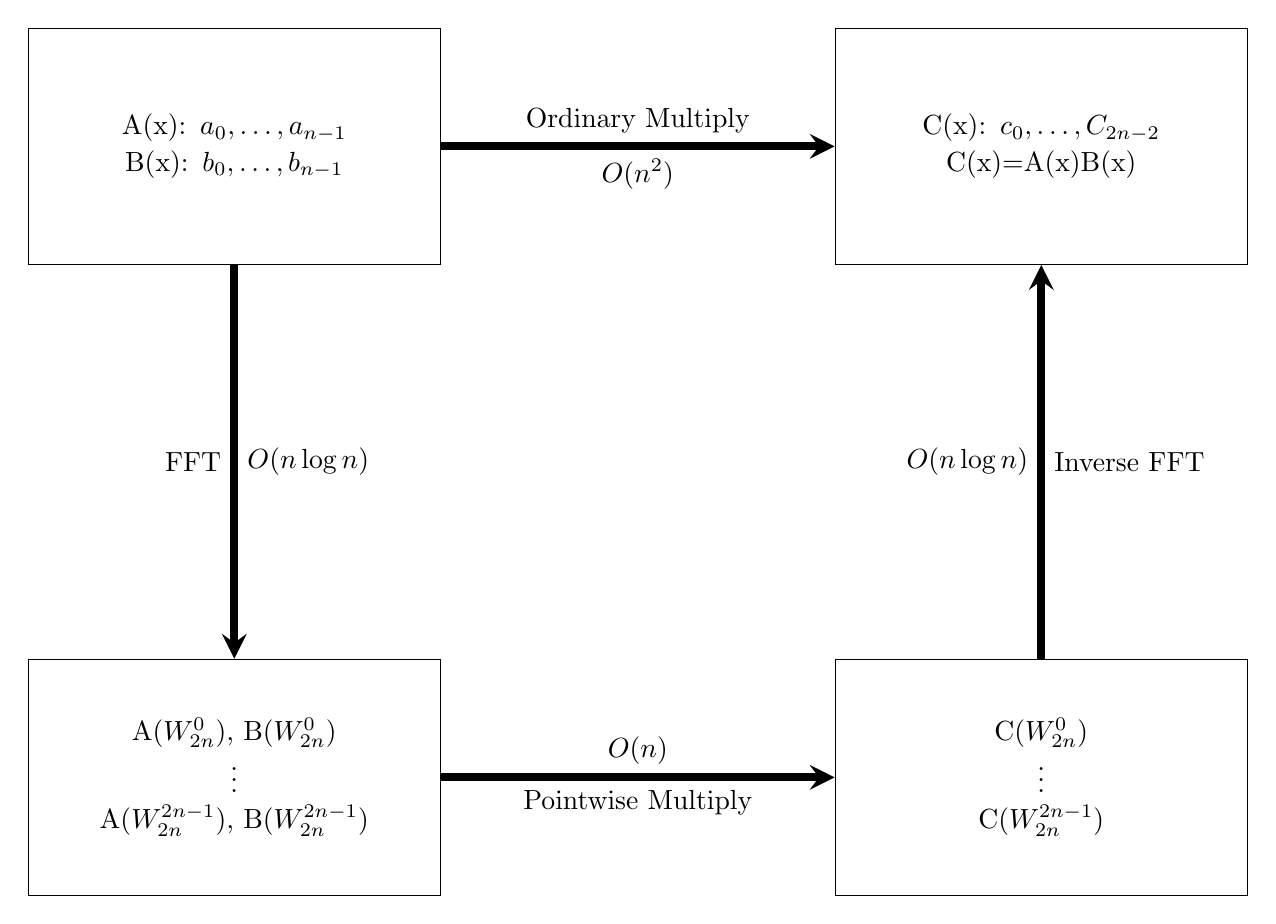
\begin{tikzpicture}[auto, node distance=5cm, box/.style={draw, rectangle, align=center, text width=5cm, minimum height=3cm, minimum width=5cm}, arrow/.style={draw, -stealth, line width=1mm}]
    % nodes
    \node[box] (A) {A(x): $a_0, \ldots, a_{n-1}$\\B(x): $b_0, \ldots, b_{n-1}$};
    \node[box] (B) [right=of A] {C(x): $c_0, \ldots, C_{2n-2}$\\C(x)=A(x)B(x)};
    \node[box] (C) [below=of A] {A($W_{2n}^0$), B($W_{2n}^0$)\\$\vdots$\\A($W_{2n}^{2n-1}$), B($W_{2n}^{2n-1}$)};
    \node[box] (D) [below=of B] {C($W_{2n}^{0}$)\\$\vdots$\\C($W_{2n}^{2n-1}$)};

    % arrows
    \draw[arrow] (A) -- node[above, draw=none] {Ordinary Multiply} node[below, draw=none] {$O(n^2)$} (B);
    \draw[arrow] (A) -- node[left, draw=none] {FFT} node[right, draw=none] {$O(n \log n)$} (C);
    \draw[arrow] (C) -- node[above, draw=none] {$O(n)$} node[below, draw=none] {Pointwise Multiply} (D);
    \draw[arrow] (D) -- node[left, draw=none] {$O(n \log n)$} node[right, draw=none] {Inverse FFT} (B);
\end{tikzpicture}

\textsf{In this problem, we take the coefficients of two polynomials A(x) and B(x) each with a degree of $n-1$ at the most, and we want to multiply them to get C(x). Instead of using ordinary multiplication which is $O(n^2)$, we can use the FFT polynomial multiplication algorithm to get a better efficiency.}

\subsection{Algorithm: Polynomial-Multiplication-FFT}
\noindent
\textbf{Input:} \\
$a = (a_0, ..., a_{n-1})$ \\
$b = (b_0, ..., b_{n-1})$

\vspace{10pt}

\noindent
\textbf{Output:} \\
$c = (c_0, ..., c_{2n-2})$

\vspace{10pt}

\noindent
\textbf{Algorithm Steps:}
\begin{enumerate}
    \item Run FFT(a, $\omega_{2n}$) and FFT(b, $\omega_{2n}$) to get $A(x)$ and $B(x)$ at the $(2n)^{th}$ roots of unity.
    \item Multiply to get $C(x) = A(x)B(x)$ at the $(2n)^{th}$ roots of unity.
    \item Run InverseFFT(C) to get $c = (c_0, ..., c_{2n-2})$.
\end{enumerate}

\vspace{10pt}

\subsection{Algorithm: FFT}
\noindent
\textbf{Input:} \\
$a = (a_0, ..., a_{n-1})$ \\
$\omega$, an $n^{th}$  root of unity

\vspace{10pt}

\noindent
\textbf{Output:} \\
$A(\omega^0),A(\omega^1),...,A(\omega^{n-1})$

\vspace{10pt}

\noindent
\textbf{Algorithm Steps:}
\begin{enumerate}
    \item if $\omega=1$, return $A(1)$
    \item Let $a_{even}=(a_0,a_2,...,a_{n-2})$ and $a_{odd}=(a_1,a_3,...,a_{n-1})$
    \item $(s_0,s_1,...,s_{\frac{n}{2}-1})=FFT(a_{even},\omega^2)$
    \item $(t_0,t_1,...,t_{\frac{n}{2}-1})=FFT(a_{odd},\omega^2)$
    \item For $j = 0 \xrightarrow{} \frac{n}{2} - 1$
    \begin{itemize}
        \item $r_j=s_j+\omega^jt_j$
        \item $r_{\frac{n}{2}+j}=s_j-\omega^jt_j$
    \end{itemize}
    \item Return $(r_0,r_1,...,r_{n-1})$
\end{enumerate}
\textsf{NOTE: in the above algorithm, $r_j$ represents $A(\omega^j)$, and $r_{\frac{n}{2}+j}$ represents $A(\omega^{j+\frac{n}{2}})$}

\section{Matrix View of FFT}

%FOR SCRIBES: ---------- End Scribing, begin biblio -----------------
%FOR SCRIBES: The first citation is just for telling you the style. Replace
%FOR SCRIBES: this with your citations if any. If there are no citations, just
%FOR SCRIBES: remove the bib environment.


%\bibliographystyle{plain}
%\begin{thebibliography}{10}
%\bibitem{mr:random}
%R.~Motwani and P.~Raghavan.
%\newblock {\em Randomized Algorithms}.
%\newblock Cambridge University Press, 1995.
%\end{thebibliography}

\end{document}
